\section{Mobile applications}
In recent years mobile applications have become increasingly popular in many domains, such as business, health and entertainment. According to the 2015 mobile app report \cite{ComScore}, the time spent on mobile devices grew up from 51 \% in share spent time to a 62 \%, leaving the share spent time of desktop on a 38 percent and becoming the number one of digital media consumption in 2015. Also, the usage of apps which include health or tracking functions was unknown until 2014 when several apps experienced a huge growth of up to 922 percent each year\cite{ComScore}. 

Mobile devices have reached a point where their hardware capabilities are comparable to a desktop computer capabilities in terms of processing power and RAM. Furthermore, they provide added functions that are unimaginable for a desktop computer such as GPS, accelerometer and the ability to be carried throughout the day. This enables new ways of living and interacting with technology as well as bringing closer the idea of ubiquitous computing, "perhaps ubiquitous computing is already here, but took a form other than that which had been envisioned." \cite{Bell2007}. 

\begin{figure}[h]
\begin{adjustbox}{width=.4\textwidth,center=\textwidth}
  \centering
  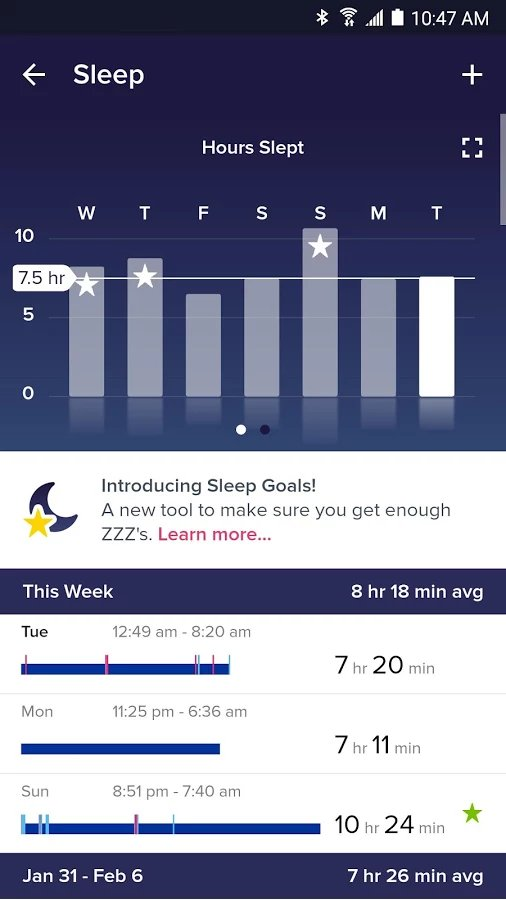
\includegraphics[scale=.5]{images/sleep_tracking.jpg}
\end{adjustbox}
  \caption[Fitbit application sleep tracking]{Fitbit application sleep tracking \footnote{\url{https://www.google.com/fit/}}}
  \label{fig:google_fit}
\end{figure}

Example of emerging applications that heavily rely on new devices hardware's capabilities, are Google Fit, \footnote{\url{https://www.google.com/fit/}} Nike +, \footnote{\url{http://www.nike.com/us/en_us/c/nike-plus/running-app-gps}} Fitbit, \footnote{\url{https://www.fitbit.com/uk}} Jawbone Up \footnote{\url{https://jawbone.com/up}} and Garmin Connect. \footnote{\url{https://connect.garmin.com/en-US/}} These apps make use of sensors that despite being simple and cheap are able to measure a range of personal activities. Such activities range over time and quality of sleep, calories ingested during the day, average heart rate of a run or steps taken during a city walk. According to Morrison et al. \cite{Rooksby2014} these people count and measure areas of their life to optimise behaviour as desired.

Recent research \cite{Barkhuus2011} suggests that people use mobile applications in personalised or individual manners, adapting functions to meet their priorities adding new functions to create their own unique experiences based on their everyday lives. There is an enormous opportunity for crafting new applications that can not only  give unique and valuable experiences but influence the way people do things in the real world. 


